\documentclass{article}

\author{John Min}


\usepackage[margin=0.5in]{geometry}
\usepackage{amssymb, amsmath, parallel, mathtools, graphicx, array, pdfpages}

\newcommand{\norm}[1]{\Vert #1 \Vert}
\newcommand{\Rn}{\R^n}
\newcommand{\Rm}{\R^m}
\newcommand{\R}{{\mathbb{R}}}
\newcommand{\grad}{\nabla}
\newcommand{\Rnn}{\R^{n\times n}}
\newcommand{\map}[3]{#1:#2\rightarrow #3}
\newcommand{\half}{\frac{1}{2}}
\newcommand{\Rmn}{\R^{m\times n}}
\newcommand{\tpose}[1]{#1^{\scriptscriptstyle T}}
\newcommand{\indicator}[2]{\delta\left(#1 \mid #2 \right)}

\title{A Deep Learning Primer: From Perceptrons to Deep Networks}

\begin{document}

\maketitle

\section{Perceptron}

In 1957, the perceptron was invented as one of the earliest supervised learning algorithms.  Now, a fundamental building block of neural networks, the perceptron is a linear, binary classifier.\\

\section{Autoencoder}
An \textbf{autoencoder}, also known as an autoassociator or Diabolo network, is an artificial neural network used for learning efficient codings, a compressed, distributed representation of the data to reduce dimensionality.  Autoencoders are comprised of at least three layers: an input layer, an output layer, and hidden layers constituting the encoding.\\

\noindent
If the neurons are linear or the single hidden layer is sigmoid, then, the optimal solution is strongly related to principal component anaalysis (PCA).


\section{Stacked Autoencoders}
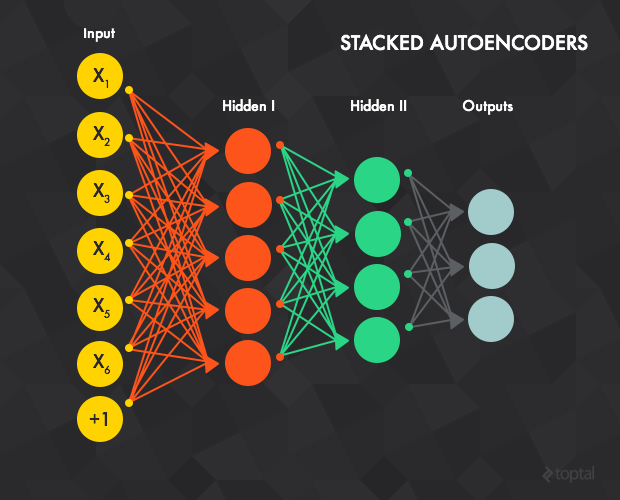
\includegraphics[scale=0.5]{Stacked_Autoencoders.png} \\

\noindent
The hidden layer of autoencoder $t$ acts as an input layer to autoencoder $t+1$.



\section{Feed-Forward Neural Network}

The \textbf{Universal approximation theorem} states that a feed-forward neural network with a single hidden layer containing a finite number of neurons (a multilayer perceptron) can approximate continuous functions on compact subsets of $\mathbb{R}^n$.

\section{Hopfield Nets}
A \textbf{Hopfield network} is composed of binary threshold units with recurrent connections between them.

\begin{itemize}
	\item symmetric connections $\Rightarrow$ global energy function
	\item $\displaystyle E = - \sum_i s_i b_i - \sum_{i < j} s_i s_j w_{ij}$
	\item Energy gap = $\displaystyle \grad E_i = E(s_i = 0) - E(s_i = 1) = b_i + \sum_j s_j w_{ij}$
\end{itemize}

\subsection{Settling to an energy minimum}
\subsection{Storage capacity}






\section{Boltzmann Machine}
A \textbf{Boltzmann machine} is a stochastic recurrent neural network, the stochastic, generative counterpart of Hopfield nets.  Like a Hopfield network, a Boltzmann machine is a network of units with an energy defined for the network.  While a B.M. has binary units, what differentiates it from a Hopfield net is that the units are stochastic.  


RBM - a generative stochastic neural network that can learn a probability distribution over its set of inputs




\section{Restricted Boltzmann Machine}
Restricted Boltzmann Machines are a variant of Boltzmann machines with the constraint that neurons form a bipartite graph.  RBMs are composed of a hidden, visible, and bias layer.  (There is only one layer of hidden units).  Each edge in an RBM must connect a visible unit to a hidden unit.  (By contrast, "unrestricted" Boltzmann machines may have connections between hidden units, making them recurrent networks.)  Unlike the feed-forward networks, the connections between the visible and hidden layers are undirected meaning that the values can be propogated in both the visible-to-hidden as well as hidden-to-visible directions.  The network is also fully connected (each unit from a given layer is connected to each unit in the next).  \\


\subsection{Energy-Based Models (EBM)}

\textbf{Energy-based models} associate a scalar energy to each configuration of the variables of interest.  \footnote{Energy is synonymous for objective, loss, cost, or utility.}  Learning corresponds to modifying the energy function such that its shape has desirable properties; for example, configurations to have low energy (minimization).  Energy-based probabilistic models define a probability distrubution through an energy function, as follows:
$$p(x) = \frac{e^{-E(x)}}{Z}$$.

\noindent
The normalizing factor $Z$ is the \textbf{partition function} in the context of physical systems.
$$Z = \displaystyle \sum_x e^{-E(x)}$$

\noindent
An energy-based model can be learnt by performing (stochastic) gradient descent on the empirical negative log-likelihood of the training data.  As for the logistic regression, we will first define the log-likelihood and then the loss function as being he negative log-likelihood.
$$\mathcal{L}(\theta, \mathcal{D}) = \frac{1}{N} \displaystyle \sum_{x^{(i)} \in \mathcal{D}} \log p(x^(i))$$
$$\ell(\theta, \mathcal{D}) = -\mathcal{L}(\theta, \mathcal{D})$$

\noindent
Use the stochastic gradient $- \frac{\partial \log p(x^(i))}{\partial \theta}$ where $\theta$ are the model parameters

\subsection{Contrastive Divergence algorithm}
Hinton, 2002
Training Products of Experts by Minimzing Contrastive Divergence - renormalizing product of probability distributions aka individual experts - 
minimizing contrastive divergence is much easier to infer than maximizing data likelihood on PoE - latent variables of different experts are conditionally independent



The single-step contrastive divergence algorithm (CD-1)

\begin{enumerate}
	\item Positive phase

	\item Negative phase

	\item Weight update

\end{enumerate}

\subsection{Issues with using Reconstruction Error}


\section{Deep Belief Networks}
As with autoencoders, we can also stack Boltzmann machines to create a class of networks known as deep belief networks (DBNs).

Deep Belief nets \\
http://www.cs.toronto.edu/~hinton/absps/fastnc.pdf \\

\section{Convolutional Nets (LeNet)}
Convolutional Neural Networks (CNN) are a special class of feed-forward neural networks that are widely used in image recognition. Analogous to other neural networks, they are trained using the back-propagation algorithm. What differentiates convolutional nets from others is the architecture.  \\

\noindent
Inspired from biology, this multi-layer perceptron variant originates from research on the complex arrangement of cells within the visual cortex.

\noindent
Before diving into the architecture of a convolutional neural net, let's define an image \emph{filter}, a square region with associated weights.  A filter is applied across an entire input image, and you often apply multiple filters.  \\

\noindent
\textbf{Convolutional layers} apply a number of \emph{filters} to the input.  The result of one filter applied across the image is called a \emph{feature map}(FM) and the number of feature maps is equivalent to the number of filters. \\

The intuition behidn the shared weights acros the image is that the features will be detected regardlesss of their location, while the multiplicity of filters allows each of them to detect different sets of features.

\noindent
\textbf{Subsampling layers} reduce the size of the input.  Popular ways to subsample are the following:
\begin{itemize}
	\item max pooling
	\item average pooling
	\item stochastic pooling
\end{itemize}


\noindent
This architecture enables convolutional nets to recognize patterns with extreme variability and with robustness to distortions and simple geometric transformations aka translation invariance.\footnote{Yann LeCun's LeNet on the MNIST dataset} \\

\subsection{Max-Pooling}
\textbf{Max Pooling} is a form of non-linear down-sampling, partitioning the input image into a set of non-overlapping rectangles and for each sub-region, outputting the maximum value.  This reduces the computational complexity for upper layers and providing a form of translation invariance.  

\begin{center}
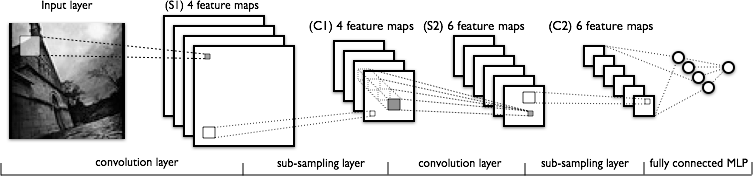
\includegraphics{mylenet.png}
\end{center}

\section{Recurrent Neural Networks}
A \textbf{recurrent neural network} (RNN) is a class of neural network where connections between units form a directed cycle.  






\end{document}
